\documentclass[../../statistical_learning_notes.tex]{subfiles}
\begin{document}
%%%%%%%%%%%%%%%%%%%%%%%%%%%%%%%%%%%%%%%%%%%%%%%%%%%%%%%%%%%%%%%%%%%%%%%%%%%
\section{Expectation Maximization}
EM is a general procedure to solve for intractable likelihood values in case of latent variables. The most general use of EM algorithm is in Gaussian Mixture Models in section \ref{sec:gmm_algo}.


%%%%%%%%%%%%%%%%%%%%%%%%%%%%%%%%%%%%%%%%
\subsubsection*{Jensen's Inequality}
Jensen's inequality is valid for concave functions. A function $f(x)$ is concave if
\begin{align*}
    f(\alpha a + (1-\alpha)b) \geq \alpha f(a) + (1-\alpha)f(b) \quad \forall \; a, b, 0 \leq \alpha \leq 1
\end{align*}

and the same inequality can be extended to arbitrary number of points
\begin{align*}
    f(\sum_{j=1}^{N} \alpha_{j}x_{j}) \geq \sum_{j=1}^{N} \alpha_{j} f(x_{j}), \quad \sum_{j=1}^{N} \alpha_{j} = 1
\end{align*}

Since the $\alpha$ in the above formula sum upto $1$, we can interpret them as a probability distribution. Let $p(t_{j} = x_{j}) = \alpha_{j}$. Then,
\begin{align*}
    f \bigg(\sum_{j=1}^{N} p(t_{j} = x_{j})x_{j} \bigg) &\geq \sum_{j=1}^{N} p(t_{j} = x_{j}) f(x_{j})\\
    \Aboxed{f(E_{p}[t]) &\geq E_{p}f(t)} \quad \text{if $f$ is concave}
\end{align*}
or, the function of expected value is greater than or equal to the expected value of the function.


%%%%%%%%%%%%%%%%%%%%%%%%%%%%%%%%%%%%%%%%
\subsubsection*{Kullback Leibler Divergence}
KL Divergence is a method to measure the difference between two probability distributions. For two probability distributions $p$ and $q$
\begin{align*}
    \Aboxed{\KL{q}{p} = \int q(x) log\frac{q(x)}{p(x)} dx}
\end{align*}

where the right side is expectation of the logarithm under the probability distribution $q(x)$. It has the following properties
\begin{enumerate}
    \item $\KL{q}{p} \neq \KL{p}{q}$ and is thus not a strict distance metric
    \item $\KL{q}{q} = 0$
    \item $\KL{q}{p} \geq 0$
\end{enumerate}
The last equation can be proved as follows
\begin{gather*}
    -\KL{q}{p} = -E_{q} \bigg[log \frac{q}{p} \bigg] = E_{q} \bigg[log \frac{p}{q} \bigg]\\
    E_{q}\bigg[ log\frac{p}{q} \bigg] \leq log \bigg( E_{q} \bigg[\frac{p}{q} \bigg] \bigg) = log \bigg(\int q(x) \frac{p(x)}{q(x)} dx \bigg) = 0\\
    -\KL{q}{p} \leq 0\\
\end{gather*}
where the second line uses Jensen's inequality and also the fact that $\int p(x) dx = 1$.


\paragraph{EM} Now we discuss the general form of the EM algorithm. Consider the problem of obtaining the MLE of data set $X$ containing $N$ data points
\begin{align*}
    p(X|\theta) &= \prod_{i=1}^{N} p(x_{i}|\theta)\\
    log(p(X|\theta)) &= \sum_{i=1}^{N} log(p(x_{i}|\theta))
\end{align*}

Assume we have some latent variables $z_{i}$ such that knowing those will make the optimization of the log likelihood easier. EM shines in such scenarios. Marginalising over $z$
\begin{align*}
    log(p(X|\theta)) &= \sum_{i=1}^{N} log \bigg(\sum_{z_{i}} p(x_{i}, z_{i}|\theta) \bigg)
\end{align*}

Assume a probability distribution $Q_{i}(z)$ (also called variational distribution) on $z$ such that $\sum_{z} Q_{i}(z) = 1$ and $Q_{i}(z) \geq 0$
\begin{align*}
    log(p(X|\theta)) &= \sum_{i=1}^{N} log \bigg( \sum_{z_{i}} Q_{i}(z_{i}) \frac{p(x_{i}, z_{i}|\theta)}{Q_{i}(z_{i})} \bigg)\\
    log(p(X|\theta)) &\geq \sum_{i=1}^{N} \sum_{z_{i}} Q_{i}(z_{i}) log \frac{p(x_{i}, z_{i}|\theta)}{Q_{i}(z_{i})} = \mathcal{L}(\theta, Q)
\end{align*}
through Jensen's inequality ($Q(z)$ is a probability distribution).\newline

Thus, we have found a lower bound on the likelihood that is now a function of both $\theta$ and $Q$. We wish to find a suitable maxima to this term that can help us find the maxima of the original likelihood function. The critical concept to know here is that if we knew $Q$, we could maximize and get the $\theta$ and vice versa. Hence, we break down the EM algorithm into two alternating steps
\begin{itemize}
    \item Expectation step : Fix $\theta^{(k)}$ and maximize $\mathcal{L}(\theta^{(k)},Q)$ to get $Q^{(k+1)}$
    \item Maximization step : Fix $Q$ and maximize $\mathcal{L}(\theta, Q^{(k+1)})$ to get $\theta^{(k+1)}$
\end{itemize}

\begin{figure}[h]
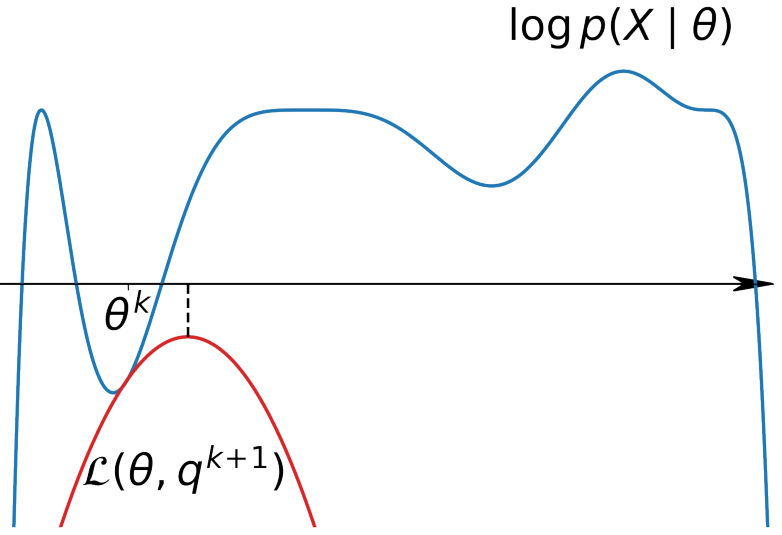
\includegraphics[scale=0.5]{em_1}
\centering
\caption{Optimal choice for $Q$ distribution at E-step in EM makes the lower bound touch the log likelihood function (1-d representation for simplicity)}
\label{fig:em_1} %\ref{fig:em_1}
\end{figure}

Now note that $Q$ is not explicitly known to us, and we define it in a special way so that the Jensen's inequality holds exactly at the equality point when $\theta$ is fixed. This will make the log likelihood exactly equal to the lower bound, and the curves for log likelihood and lower bound would touch at this fixed $\theta$ (fig \ref{fig:em_1}). Thus,
\begin{align*}
    log(p(X|\theta)) &= \sum_{i=1}^{N} \sum_{z_{i}} Q_{i}(z_{i}) log \frac{p(x_{i}, z_{i}|\theta)}{Q_{i}(z_{i})}\\
    0 &= log(p(X|\theta)) - \sum_{i=1}^{N} \sum_{z_{i}} Q_{i}(z_{i}) log \frac{p(x_{i}, z_{i}|\theta)}{Q_{i}(z_{i})}\\
    &= \sum_{i=1}^{N}log(p(x_{i}|\theta)) \times 1 - \sum_{i=1}^{N} \sum_{z_{i}} Q_{i}(z_{i}) log \frac{p(x_{i}, z_{i}|\theta)}{Q_{i}(z_{i})}\\
    &= \sum_{i=1}^{N}log(p(x_{i}|\theta)) \sum_{z_{i}}Q_{i}(z_{i}) - \sum_{i=1}^{N} \sum_{z_{i}} Q_{i}(z_{i}) log \frac{p(x_{i}, z_{i}|\theta)}{Q_{i}(z_{i})}\\
    &= \sum_{i=1}^{N} \sum_{z_{i}}Q_{i}(z_{i}) \bigg( log(p(x_{i}|\theta)) - log \frac{p(x_{i}, z_{i}|\theta)}{Q_{i}(z_{i})} \bigg)\\
    &= \sum_{i=1}^{N} \sum_{z_{i}}Q_{i}(z_{i}) log \frac{p(x_{i}|\theta) Q_{i}(z_{i})}{p(x_{i}, z_{i}|\theta)}\\
    &= \sum_{i=1}^{N} \sum_{z_{i}}Q_{i}(z_{i}) log \frac{p(x_{i}|\theta) Q_{i}(z_{i})}{p(z_{i}|x_{i},\theta)p(x_{i}|\theta)}\\
    &= \sum_{i=1}^{N} \sum_{z_{i}}Q_{i}(z_{i}) log\frac{Q_{i}(z_{i})}{p(z_{i}|x_{i},\theta)}\\
    &= \sum_{i=1}^{N} \KL{Q_{i}(z_{i})}{p(z_{i}|x_{i},\theta)}\\
    \text{For minima,} \quad Q_{i}(z_{i}) &= p(z_{i}|x_{i},\theta) \; \forall \; i = 1,\ldots,N
\end{align*}
since $KL$ divergence $\geq 0$ and the minimum is attained when the two distributions coincide. Thus, E-step is simply setting $Q$ to be the posterior of $z$ given $x$ and $\theta$.\newline

Moving to the M-step, we fix the value of $Q$ and maximize $\mathcal{L}(\theta, Q)$ with respect to $\theta$
\begin{align*}
    \max_{\theta}\mathcal{L}(\theta, Q) &= \max_{\theta} \sum_{i=1}^{N} \sum_{z_{i}} Q_{i}(z_{i}) log \frac{p(x_{i}, z_{i}|\theta)}{Q_{i}(z_{i})}\\
    &= \max_{\theta} \sum_{i=1}^{N} \sum_{z_{i}} Q_{i}(z_{i}) log(p(x_{i}, z_{i}|\theta)) - \sum_{i=1}^{N} \sum_{z_{i}} Q_{i}(z_{i})log(Q_{i}(z_{i}))\\
    &= \max_{\theta} E_{Q}[log(P(X, Z|\theta))]
\end{align*}
i.e., the expectation of the joint distribution of $X$ and latent variables $Z$. Usually this function is concave (we can define in such a way) and local optima are easily achievable.\newline

\subsubsection*{Convergence Guaranties}
The above described EM algorithm leads to an increase in the log likelihood at each step because of the following relations
\begin{alignat*}{2}
    log(P(X|\theta_{k})) &= \mathcal{L}(\theta_{k}, Q_{k+1}) \quad &&\text{equality case in E-step}\\
    \mathcal{L}(\theta_{k}, Q_{k+1}) &\leq \mathcal{L}(\theta_{k+1}, Q_{k+1}) \quad &&\text{M-step to maximize for $\theta$}\\
    \mathcal{L}(\theta_{k+1}, Q_{k+1}) &\leq log(P(X|\theta_{k+1})) \quad &&\text{Jensen's inequality}\\
    \text{or,} \quad log(P(X|\theta_{k})) &\leq log(P(X|\theta_{k+1}))
\end{alignat*}

\subsubsection*{EM Algorithm}
Repeat until convergence
\begin{enumerate}
    \item E-step : set $Q^{(k+1)}_{i}(z_{i}) = p(z_{i}|x_{i}, \theta^{(k)}) (= \argmin_{Q} \sum_{i=1}^{N}\KL{Q_{i}(z_{i})}{p(z_{i}|x_{i}, \theta^{(k)})}$
    \item M-step : $\theta^{(k+1)} = \argmax_{\theta} E_{Q^{(k+1)}}[log(P(X,Z|\theta))]$
\end{enumerate}
\end{document}